\documentclass{article}
\usepackage[utf8]{inputenc}
\usepackage{hyperref}
\usepackage{graphicx}
\usepackage{subfig}

\title{COMP140 Report}
\author{Christopher Robertson}
\date{March 2020}

\begin{document}

\maketitle
\begin{center}
    \href{https://github.com/Koltonix/comp140-arduino-controller}{GitHub}
\end{center}
\newpage

\section{Project Proposal}

The game design for the controller is a game where you control three sets of colours which are you able to change the hue of using a set of dials - or for debugging two keys on the keyboard. Each colour you control has a lane of queued up colours which the player must match their colour to the next colour in the lane. When the colours are matched they are able to press the dial - or a third keyboard button for debugging - to submit. The game will then either add points, or deduct lives if successful or not. As time goes on the speed of the game will increase much like any re-playable arcade game like this.

\subsection{Research and Key Components}

\subsubsection{Rotary Encoder x 3}

When looking into my design for this controller I was going to at first have a potentiometer with a button adjacent to it to act as the submit, but I felt that this wasn't very ergonomic or practical, so I decided to look for a potentiometer with a built in button, but instead found something called a rotary encoder. I found that it is often used for GUI navigation since it rotates in 360 degrees rather than the potentiometer which is limited. This will work even better for my game since it would represent a colour wheel better. \href{https://www.youtube.com/watch?v=UhYu0k2woRM}{Research Video}

\subsubsection{RGB LED Strip x 3}

Since I want a sort of built in controller I looked at LED strips to see what I could do with them and their limitations and found that you are able to get LED strips that have each programmable LEDs with the addition of RGB which is exactly what I am aiming for. Furthermore, the \ref{https://www.youtube.com/watch?v=dZZynJLmTn8}{video} also outlines how to use a pre-made library to affect the values easily. I also checked to ensure that you are able to cut the LED strips to certain lengths and for them to still work which they do.

\subsubsection{LCD Display x 1}

I was deciding whether to use an LCD display, or a 7 segment display, but ultimately decided on the former since it provides far more customisation with what I can display on the screen and plus it has more space for characters since the segment had far less which might become problematic at higher scores for my game.

\subsection{Controller Design}

I intend for the controller to be completely function by itself without the use of a screen as a sort of built in controller since it will display all of the elements using RGB LED strips. It will also display the score using either an LCD screen, or a 7 Segment Display. You are then able to control the three lane inputs with rotary encoders and submit by pressing it. Although you can play it by itself I do intend on making a Unity game to go along side it which will act as an extender to see the colours further down as well as other diagnostics and general gameplay.

\subsection{Key User Stories}

One of the main users stories would be "As a player I want to get the correct colour to gain more score" since it is the primary objective of the game for the player.

\subsection{Research and Key Components}

\subsubsection{Rotary Encoder x 3}

When looking into my design for this controller I was going to at first have a potentiometer with a button adjacent to it to act as the submit, but I felt that this wasn't very ergonomic or practical, so I decided to look for a potentiometer with a built in button, but instead found something called a rotary encoder. I found that it is often used for GUI navigation since it rotates in 360 degrees rather than the potentiometer which is limited. This will work even better for my game since it would represent a colour wheel better. Furthermore, it also has a built in button too, so I don't have to add an extra external one, but instead an extra cable.

\subsubsection{RGB LED Strip x 3}

Since I want a sort of built in controller I looked at LED strips to see what I could do with them and their limitations and found that you are able to get LED strips that have each programmable LEDs with the addition of RGB which is exactly what I am aiming for. Furthermore, the \href{https://www.youtube.com/watch?v=UhYu0k2woRM}{video} also outlines how to use a pre-made library to affect the values easily.

\subsubsection{LCD Display x 1}

I was deciding whether to use an LCD display, or a 7 segment display, but ultimately decided on the former since it provides far more customisation with what I can display on the screen and plus it has more space for characters since the segment had far less which might become problematic at higher scores for my game. Furthermore, I could also add a highscore to the LCD screen quite simply compared to the segment which would require an additional one. \href{https://www.youtube.com/watch?v=dZZynJLmTn8}{Research Reference}.

\subsection{Controller Design}

I intend for the controller to be completely function by itself without the use of a screen as a sort of built in controller since it will display all of the elements using RGB LED strips. It will also display the score using either an LCD screen, or a 7 Segment Display. You are then able to control the three lane inputs with rotary encoders and submit by pressing it. Although you can play it by itself I do intend on making a Unity game to go along side it which will act as an extender to see the colours further down as well as other diagnostics and general gameplay.

\subsection{Key User Stories}

One of the main users stories would be "As a player I want to get the correct colour to gain more score" since it is the primary objective of the game for the player.

\section{Hardware and Components}

There are two main components that I am using for this controller which is the Rotary Encoder (with an LED Light) which acts as the input and output. I also am using an RGB LED strip which only acts as the output for the player and is the primary visuals for the game experience. The other components I'll be using include the Arduino Uno board which will be processing everything and holding the sketch itself. I will also be using a breadboard too as the Arduino Uno doesn't have enough live and ground slots for me to use.

\subsection{Rotary Encoder and RGB LEDs}

\begin{figure}[ht]%
    \centering
    \subfloat[Rotary Encoder]{{\includegraphics[angle=-90, width=5cm]{rotary_encoder.jpg}}}%
    \qquad
    \subfloat[LED Strip]{{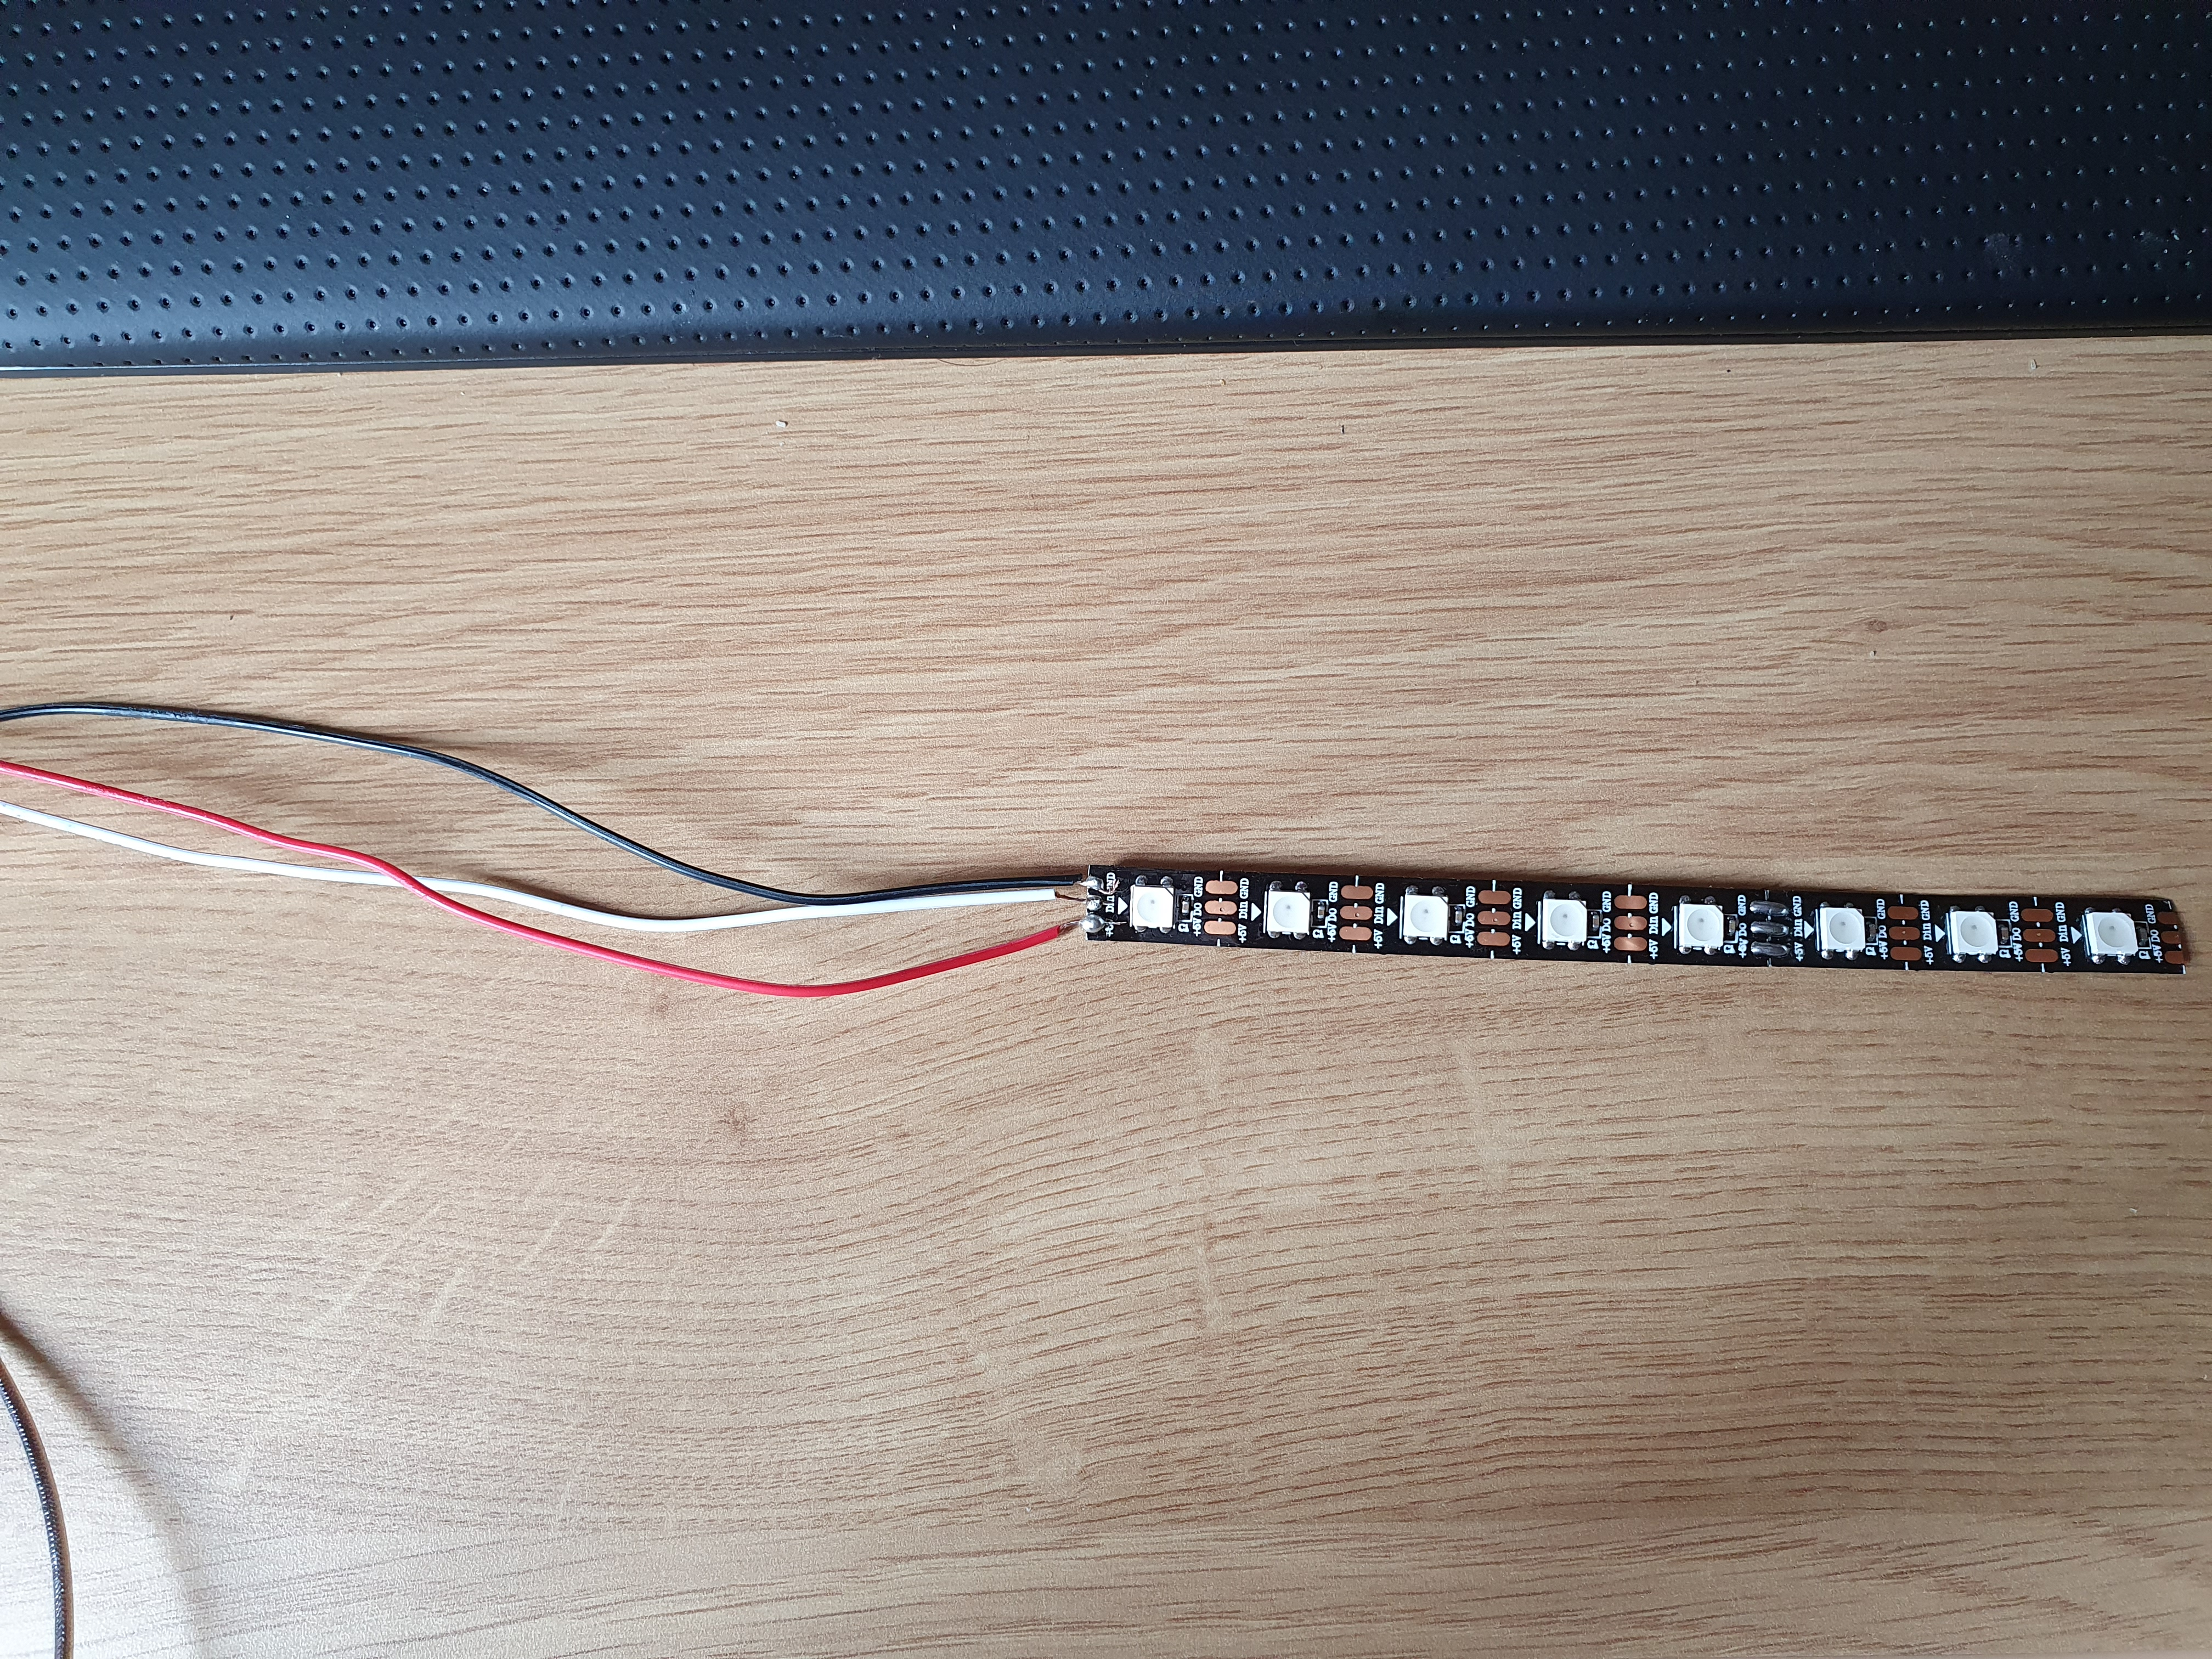
\includegraphics[angle=-90, width=5cm]{led_strip.jpg}}}%
    \caption{External Components}%
    \label{fig:external_component}%
\end{figure}

The rotary encoder is used to control the colour currently selected by rotating the dial which then cycles through an array of available colours. The player is informed of the colour selected by the RGB LED on the rotary encoder itself. Once the player thinks the selected colour is the same as the next colour they press the button to submit.
\\
\\
The LED RGB Strip is used to feedback the current state of the game to the player. It represents the queue of colours that are next in order. The player will then use the rotary encoder to match the next colour. I am then using the Adafruit Neopixel library to individually address each LED with a different colour.

\subsection{Arduino and Breadboard}

\begin{figure}[ht]%
    \centering
    \subfloat[Arduino Uno]{{\includegraphics[angle=-90, width=5cm]{arduino-uno.jpg}}}%
    \qquad
    \subfloat[Breadboard]{{\includegraphics[angle=-90, width=5cm]{breadboard.jpg}}}%
    \caption{Main Hardware}%
    \label{fig:main_hardware}%
\end{figure}

The Arduino will be the main piece of hardware in this project since it will be storing the entire game and the logic behind it. It will take in the input from the rotary encoder and then produce an output to both the rotary encoder LED and the LED strip. I will also be using a breadboard as I wouldn't have needed one if the Arduino had 3 extra 5v slots and 1 extra ground slot.

\section{Design of the Controller - Wiring, Casing and Attachments}
\subsection{Design}

\begin{figure}[ht]%
    \centering
    \subfloat[Concept]{{\includegraphics[width=5cm]{controller-concept.png}}}%
    \qquad
    \subfloat[Final]{{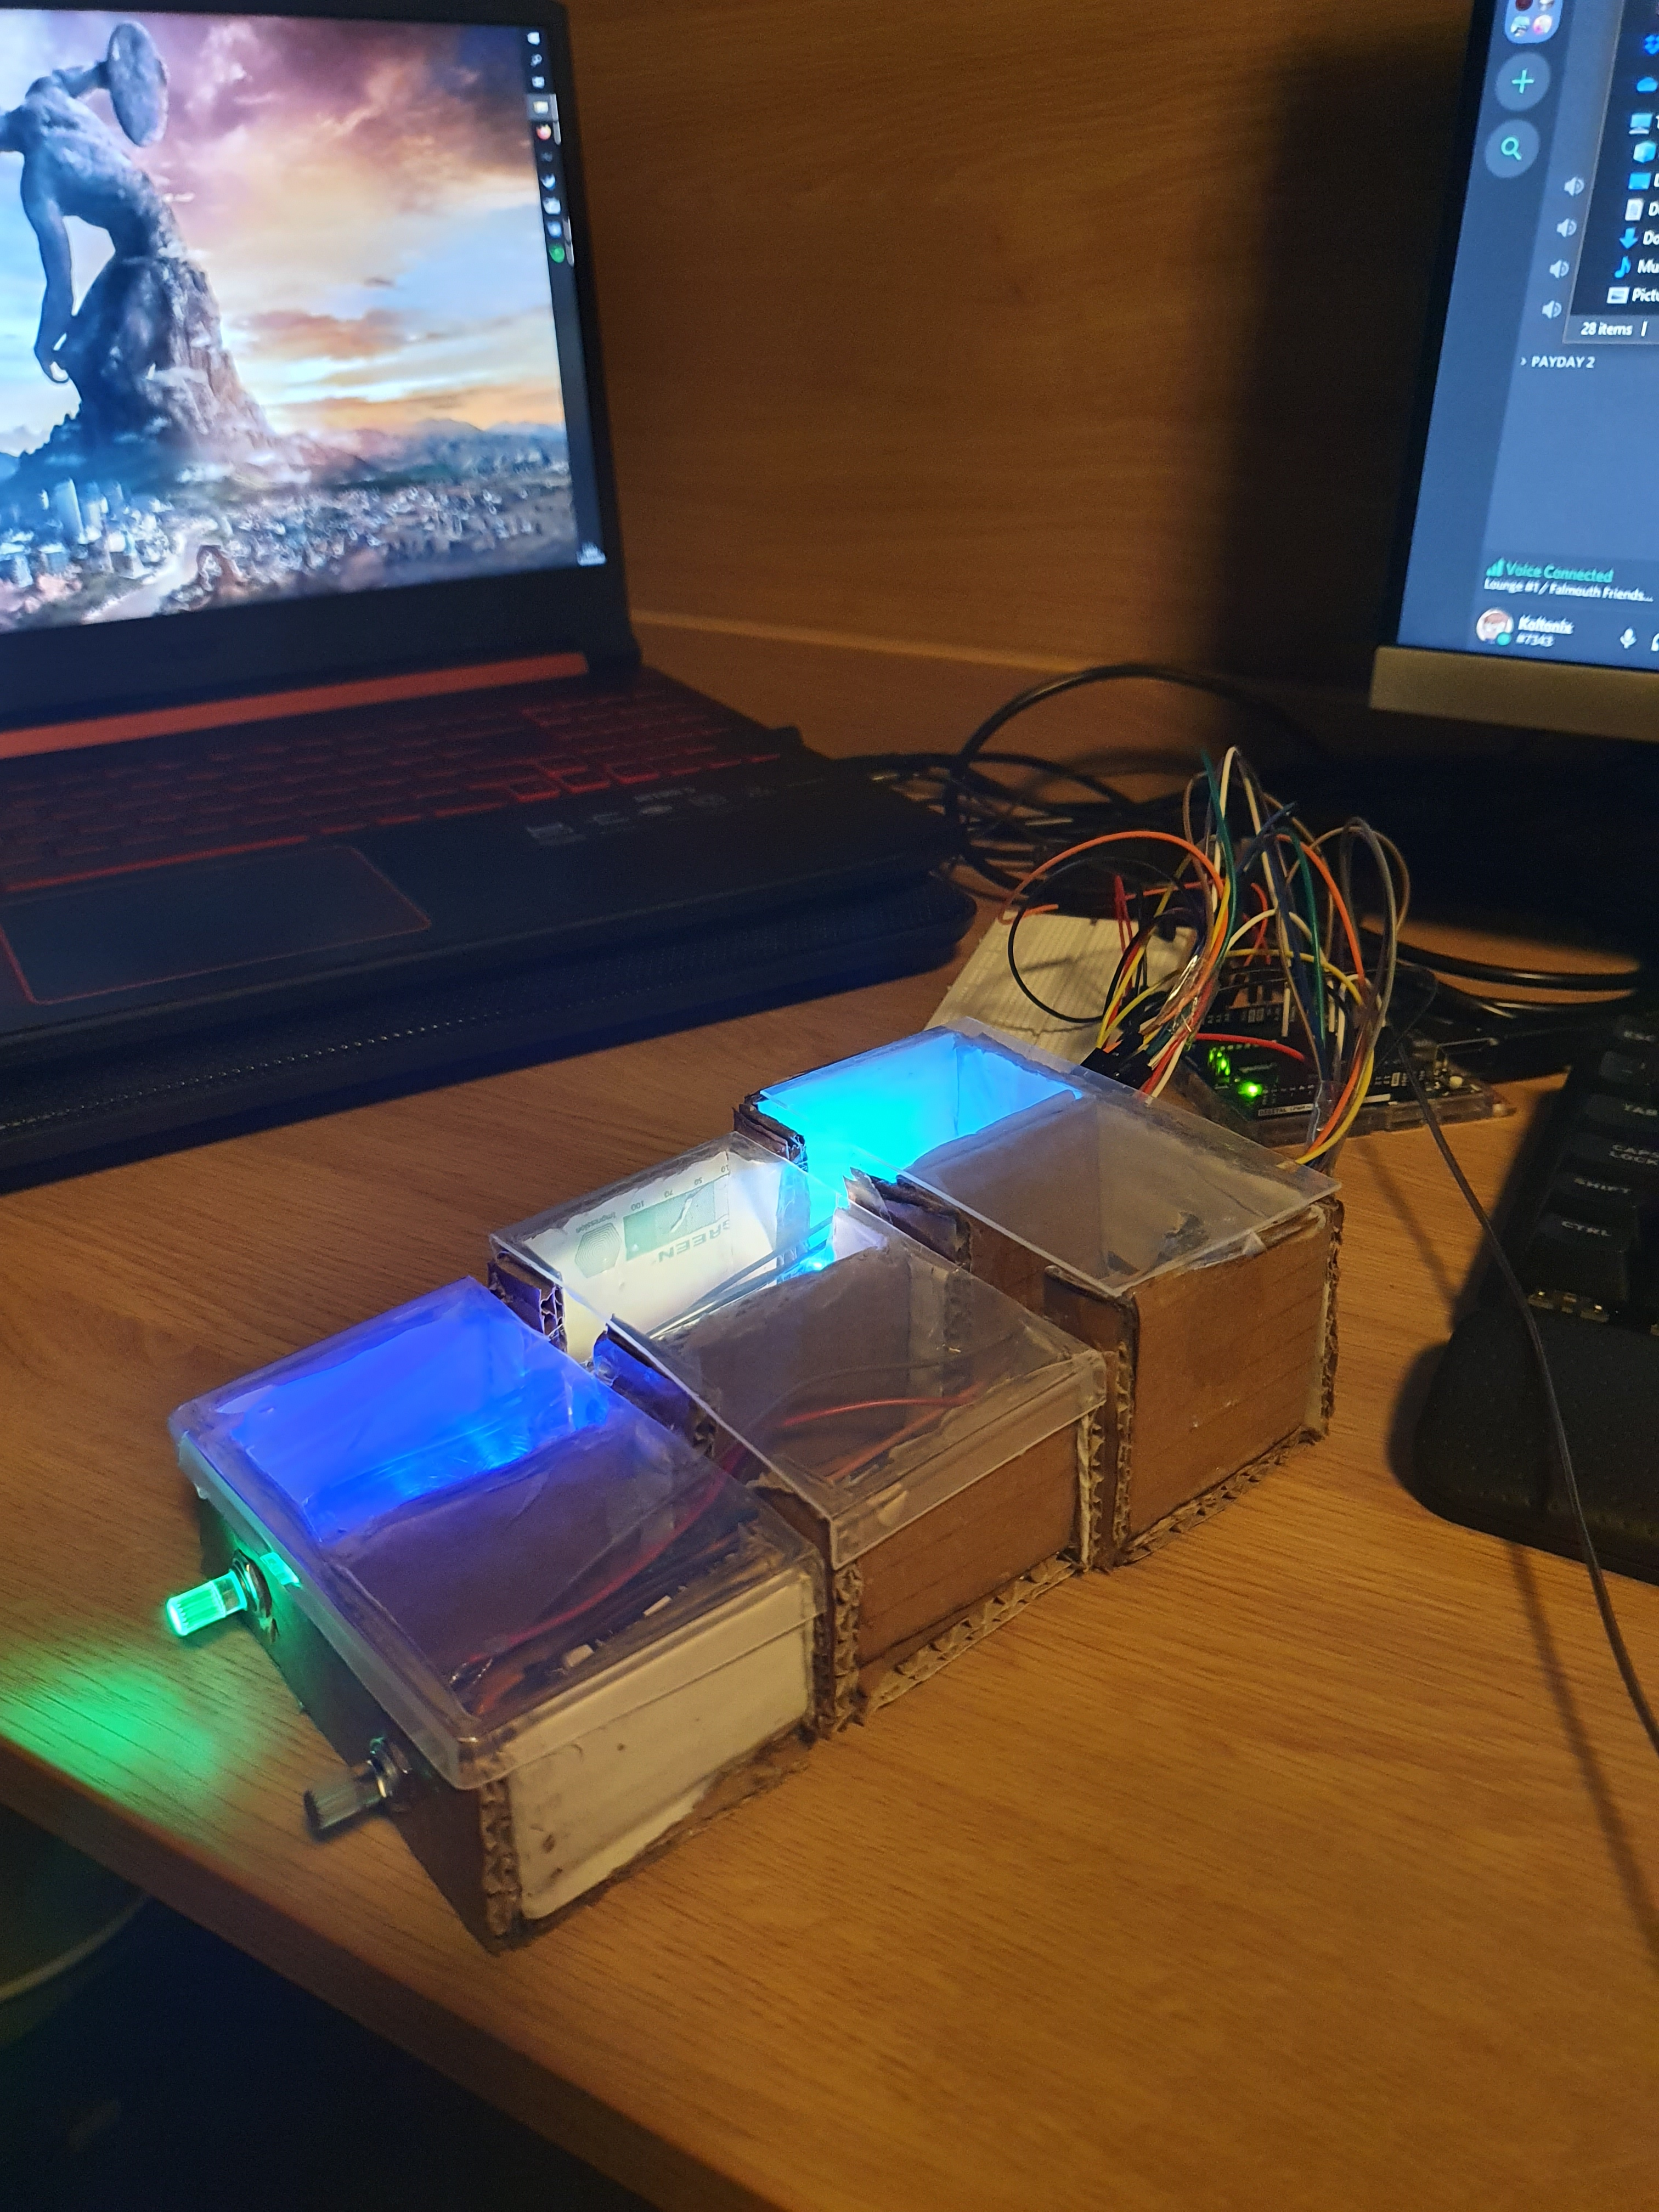
\includegraphics[width=5cm]{arduino.png}}}%
    \qquad
    \subfloat[Wiring]{{\includegraphics[width=5cm]{arduino-wiring.PNG}}}%
    \caption{Controller Design}%
    \label{fig:controller-design}%
\end{figure}

The design of my controller is to have 3 layers of boxes at 3 separate heights because I feel it is just a bit more aesthetically appealing than just being flat. The top of each of these boxes has a clear layer of plastic so that the player may see the LED colour inside. On the front are the two rotary encoders which are used to control each respective lane. I went for a simple design approach for this and tried to make it look like a sort of toy since that is the kind of game I was making with the in-built controller idea.
\\
\\
The casing of my controller is made out of thick cardboard - although plastic had been planned - where I made 3 sets of rectangular boxes with no top by cutting a sheet of cardboard and using PVA and craft glue to stick it together. Once it had dried I cut around the rough edges and then made each rectangular box its own height in descending order.

\section{Game Experience/Concept}
\begin{figure}[ht]
  \includegraphics[width=\textwidth,height=\textheight,keepaspectratio]{unity-diagnostics.PNG}
  \caption{Unity Scene}
  \label{fig:unity-diagnostics}
\end{figure}

The game itself is to use the dials to change the colour of the selected colour to match the next one in the queue and will repeat indefinitely much like any sort of arcade game and as time goes on you'll have less time to react. Although the controller will function by itself I also have a debugging game using Unity which allows you to see all of the values on the controller as well as the score since I didn't have enough space on the Arduino for the LCD screen.

\section{Software Design with UML Diagrams}

\begin{figure}[ht]%
    \centering
    \subfloat[Class Diagram]{{\includegraphics[width=5cm]{uml-class-diagram.PNG}}}%
    \qquad
    \subfloat[Sequence Diagram]{{\includegraphics[width=5cm]{uml-sequence-diagram.PNG}}}%
    \qquad
    \subfloat[Case Diagram] {{\includegraphics[width=5cm]{uml-case-diagram.png}}}%
    \caption{UML Diagrams}%
    \label{fig:uml-diagrams}%
\end{figure}

I feel that the UML Diagram that best reflects my software design is the UML Class Diagram as it shows how all of the classes interact and their respective behaviours. I've decided to go with inheritance in my planning for the input since it will allow me to use multiple different types of implementations for the input, but still get the same final value which reduces my redundancy of my code. I then also planned to use a protocol to decouple the Lane and UserInput as much as possible while still requiring the data. The Lane then processes the input data and determines the state of the current lane. From there the GameController uses 'x' amount of Lanes to process the state of the game.
\\
\\
The case diagram was also useful in representing my software on a broader scale in terms of the real world since it shows how the user interacts with the Arduino and how that translates into the software. It also represents my software design between different systems too since the Arduino will interact with the user, but also Unity separately too.
\\
\\
The sequence diagram was useful in representing the interaction of the Arduino and the user in a closer scope rather than a more broader sense like the case diagram. It also shows the data transfer between each piece of hardware and software too.

\section{Reflection}

\subsection{Arduino Ports}
In hindsight, one area would have benefit me from the would have been to look into how many ports all of my components would need since I only realised once I had the physical components that I would have too few slots for everything I needed hence the scaling back in the size of my controller and the features.
\\

\subsection{Soldering}
Another difficult area was the soldering since I had never actually done it before, but did watch a couple of videos on how to do it. Overall, I was successful in soldering; however, I didn't do the best job of it mainly due to a lack of holding equipment for the components, so in the future I'd look into buying a clamp/stand to make my life infinitely easier when soldering.
\\

\subsection{C++ in General}
Since my controller is entirely independent from any other system except the Arduino I needed to code everything in C/C++ which proved to be quite a challenge mainly due to the debugging difficulties. One example is where I spent a fair amount of hours trying to figure out a pointer issue that I was having and finally narrowed it down to an array that wouldn't work one tenth of the time; however, this project has been exceptional practice for C++. In the future, I would have probably looked into C++ a bit earlier.
\\

\subsection{C++ Arduino Libraries}
A final issue I had near the deadline was that the libraries that I had used when testing the C++ code in a separate environment. The issue with the libraries was that the Arduino didn't support them which was a problem since I relied on the queues and vectors in the their respective library, but luckily there were a variety of custom libraries that I could use to replace instead.
\end{document}
